

\section{Results}

\subsection{Part 1: Magnetic field strength and current}

\begin{figure}
    \centering
    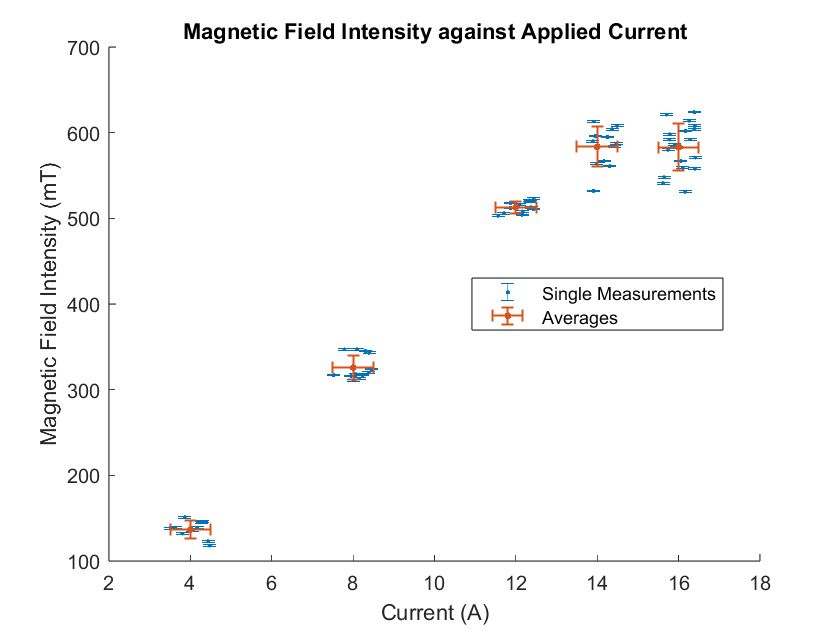
\includegraphics[width=0.8\textwidth]{Results/Figures/Magnetic_Field_vs_Current_jitter.png}
    \caption{Magnetic Field Strength vs Current Jitter Plot}
    \label{fig:magnetic_field_vs_current_jitter}
\end{figure}
\begin{figure}
    \centering
    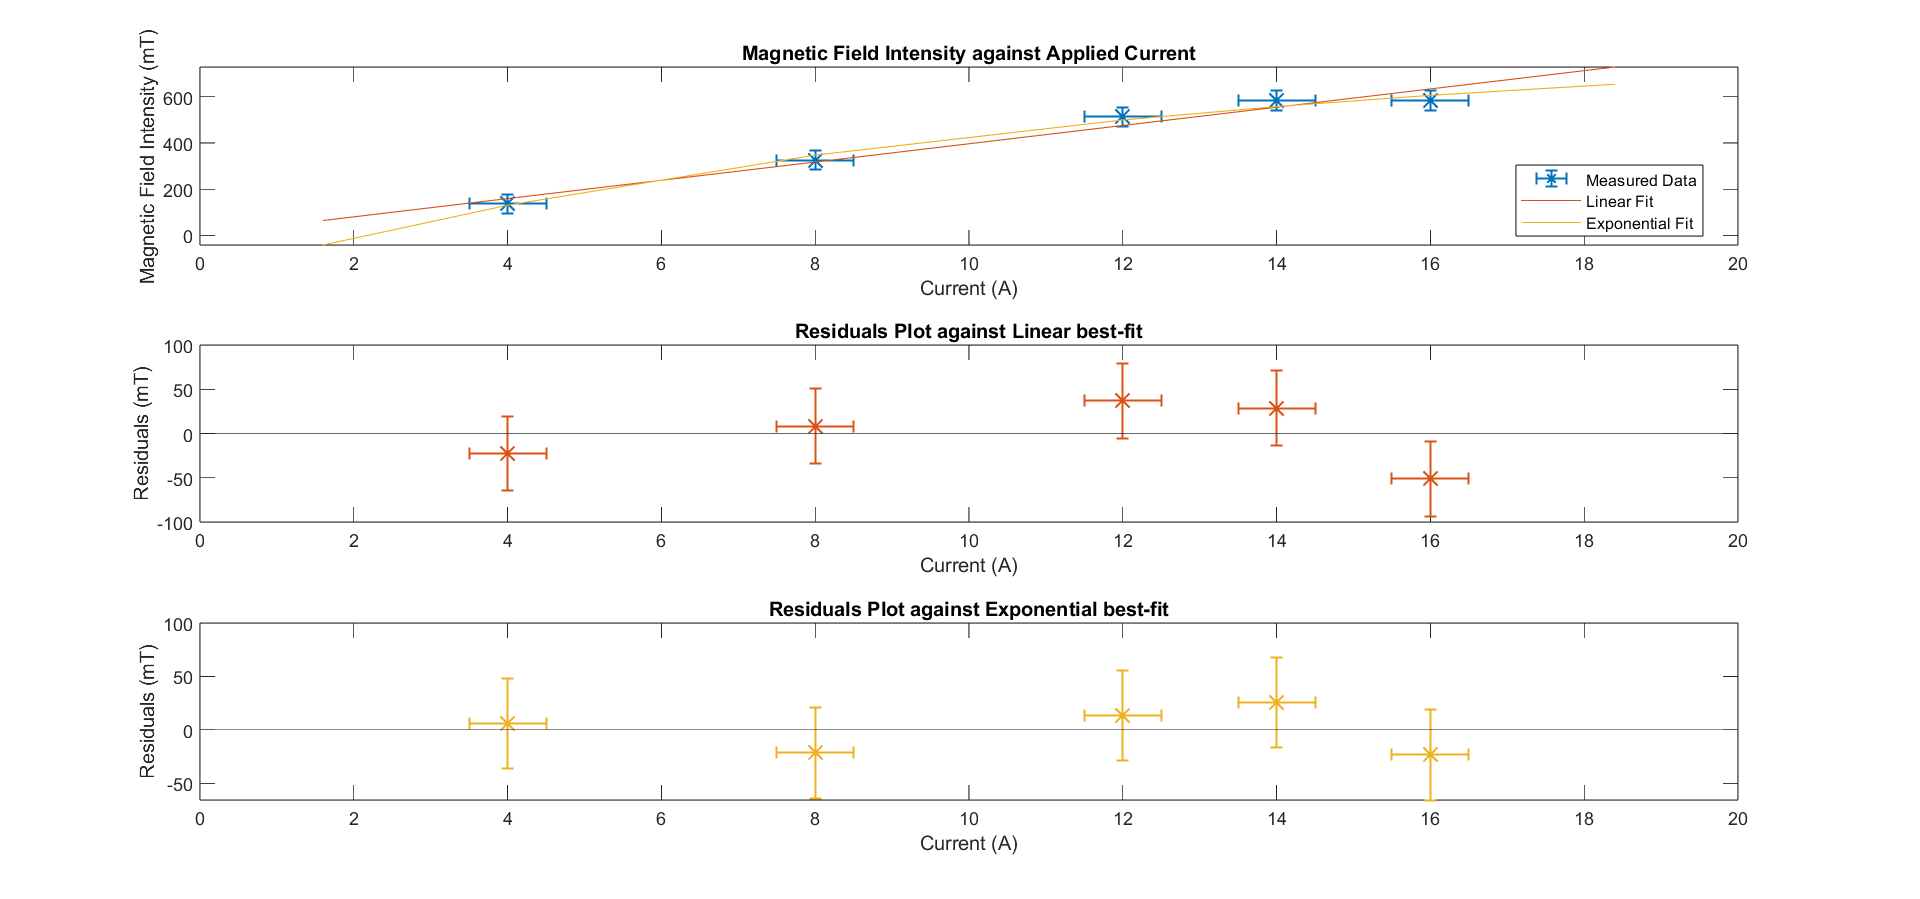
\includegraphics[width=0.8\textwidth]{Results/Figures/Magnetic_Field_vs_Current.png}
    \caption{Magnetic Field Strength vs Current Regression Plots for Linear and Exponential fits}
    \label{fig:magnetic_field_vs_current}
\end{figure}
Figure \ref{fig:magnetic_field_vs_current_jitter} shows the magnetic field strength as a function of the current supplied to the electromagnet, showing the averages and standard deviations at each measured current value. Then, using these averages, figure \ref{fig:magnetic_field_vs_current} applies a linear and exponential fit to the data. Where current I is in A, these fits are given by:
\begin{gather*}
    \text{\textbf{Linear Fit:}} \\
    B = (1 \pm 51) + (39.6 \pm 4.4)I~[mT] \quad \chi^2 / \nu = 40.0 / 3 = 13.3 \\
    \text{\textbf{Exponential Fit:}} \\
    B = (-1040 \pm 150) exp (-0.089 \pm 0.051 * I) + (860 \pm 260)~[mT] \\
    \chi^2 / \nu = 17.7 / 2 = 8.85
\end{gather*}


The linear fit has a reduced chi-squared value of 13.3, which is quite high, and the residuals show a clear downwards-curving pattern. However, the exponential fit has a lower reduced chi-squared value of 8.85 and the residuals show a more random pattern, indicating that the exponential fit is a better fit to the data than the linear fit. This may be due to there being a maximum field strength from the electromagnet, where adding more current doesn't just result in linearly increasing magnetic field strength.

\subsection{Part 2: Observing the linearity of the Zeeman shift with respect to the field strength}

Now, we plot the previously obtained values (Appendix \ref{sec:appendix} contains all of the raw measurements taken, as well as the Zeeman shift calculation for each trial organized in tables by magnetic field strength.)
in a scatter plot and compare it to a linear fit of the form $\Delta S = mB + b$.

\begin{figure}
    \centering
    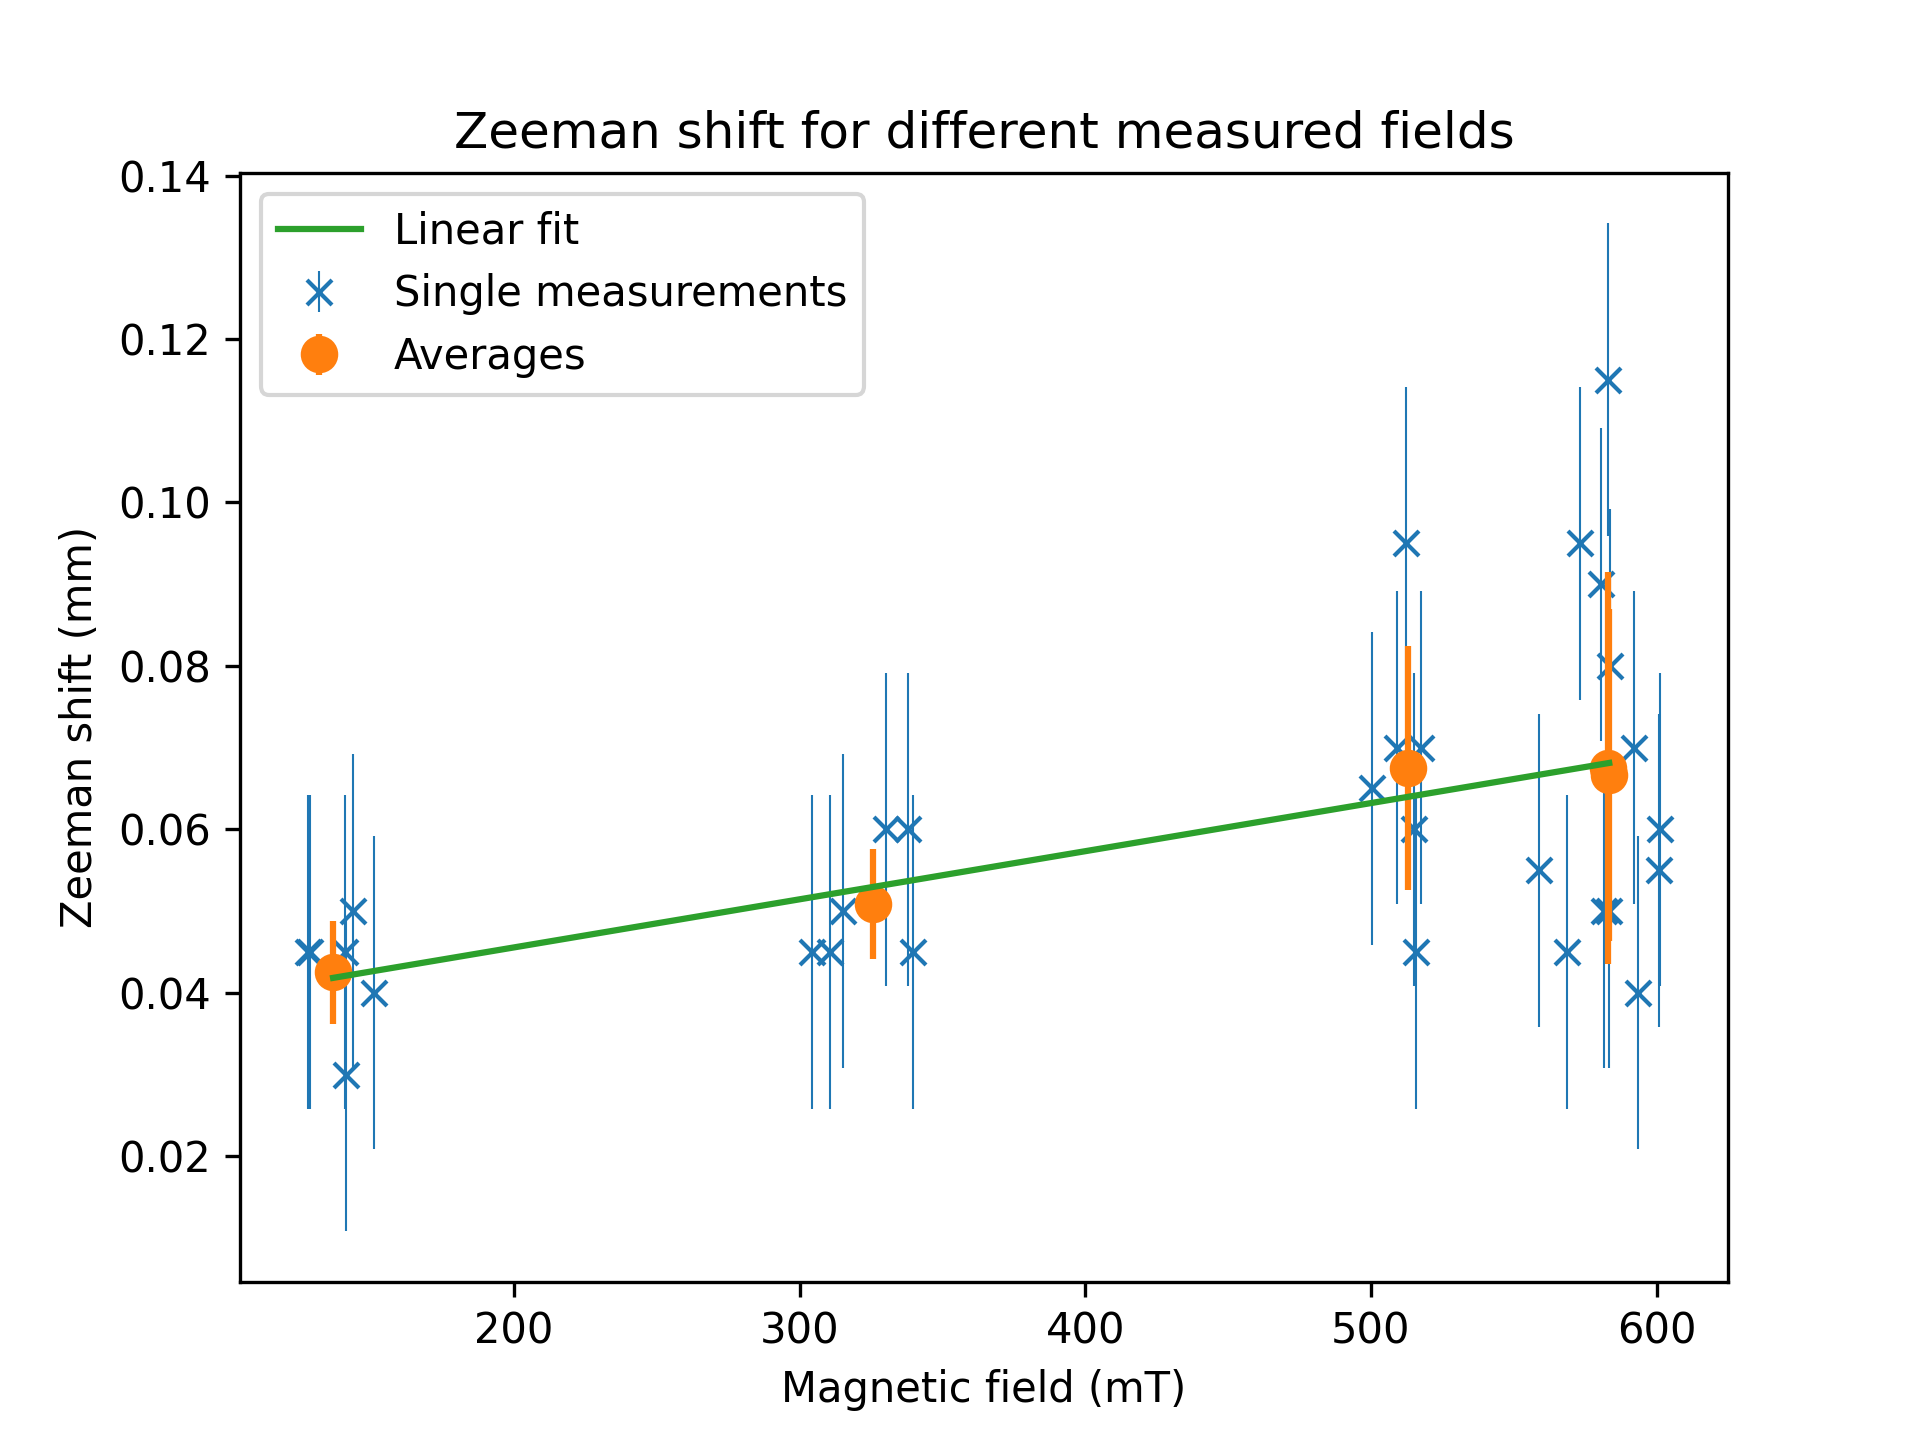
\includegraphics[width=0.8\textwidth]{Results/img/zeeman_shift_scatter.png}
    \caption{Zeeman Shift vs Magnetic Field Intensity}
    \label{fig:zeeman_shift_scatter}
\end{figure}

\begin{figure}
    \centering
    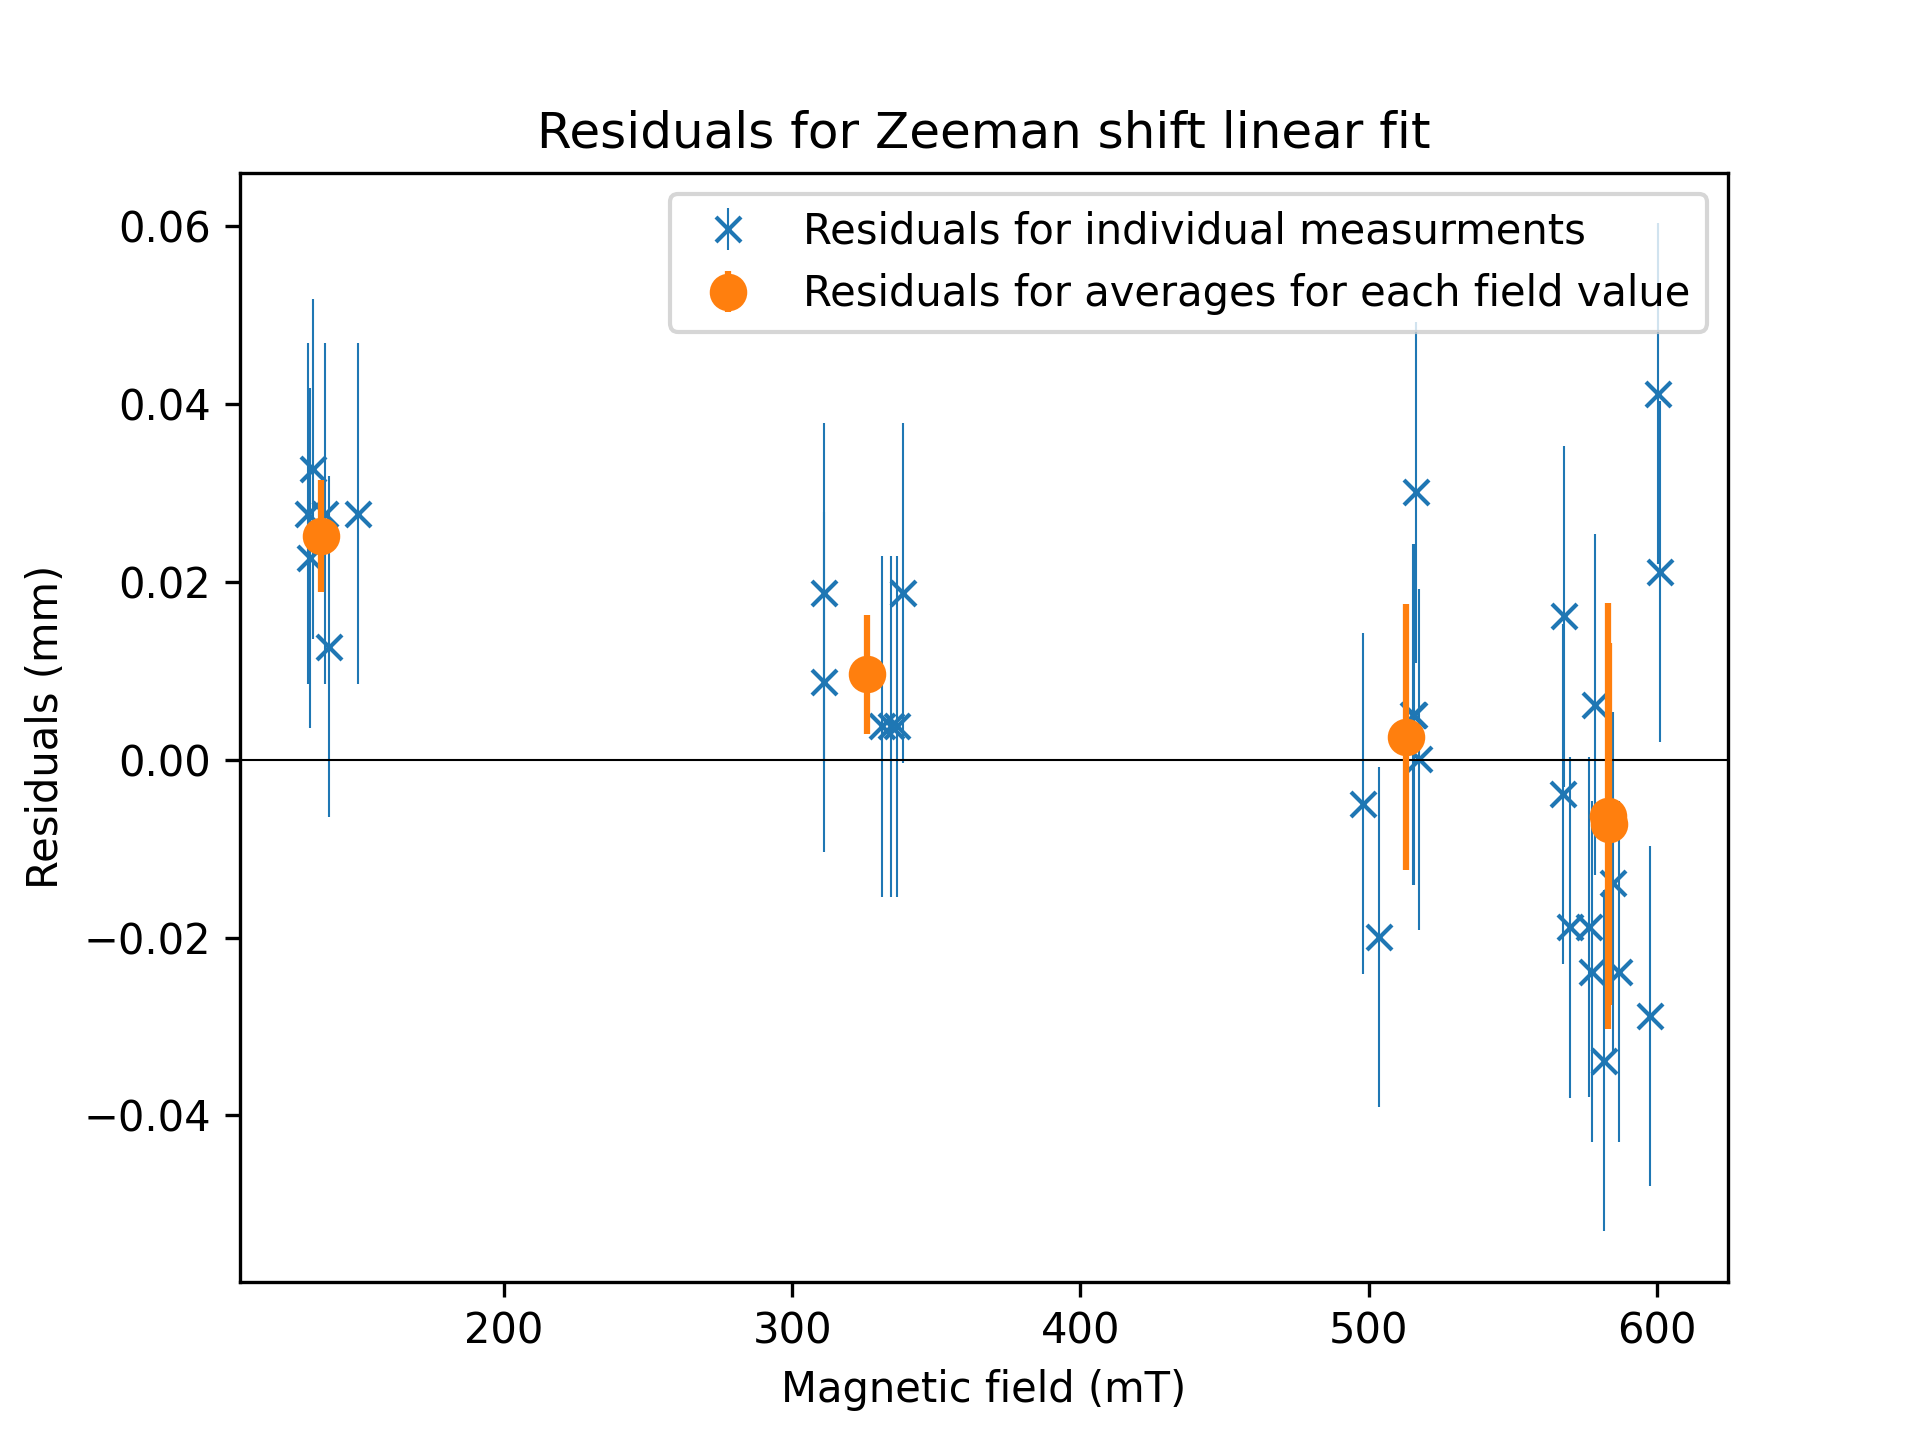
\includegraphics[width=0.8\textwidth]{Results/img/zeeman_shift_residuals.png}
    \caption{Zeeman Shift vs Magnetic Field Intensity}
    \label{fig:zeeman_shift_residuals}
\end{figure}

The parameters for the standard fit are:
\begin{gather*}
    \Delta S = (58.870 \pm 17.648)B + (33.781 \pm 8.1574) \mu m \quad \chi^2 / \nu = 114.6 / 29 = 38.2
\end{gather*}

Where B is in tesla and $\Delta S$ is in $\mu m$. The linear fit can be seen in Figure \ref{fig:zeeman_shift_scatter}, and the residuals can be seen in Figure \ref{fig:zeeman_shift_residuals}. The residuals do indicate a random
pattern above and below the line (2 of the average points are above, and the other two are below). This indicates that the linear fit is a good fit to the data.
However, the reduced Chi squared value is $38.2$, which does not indicate a good fit, since the observed uncertainties are quite large making the fit less accurate given the wide uncertainty in the residuals.
\subsection{Part 3: measuring the $\frac{e}{m}$ relationship.}

Looking back at equation \ref{eq:em_relationship}, we can see that the value of $\frac{e}{m}$ can be obtained from the slope of the linear fit of the Zeeman shift vs the magnetic field intensity in the previous section.

Before doing this, we must obtain the value of $\Delta A$ (the separation of successive interference lines). Because this quantity is not a property
of the line itself, but rather of all of the collection of lines, we obtain all of the separations for the lines without magnetic field
and then use the average of these values as a constant in this equation.

\def\lineUncertainty{0.05}
\begin{table}[h]
    \centering
    \begin{tabular}{|c|c|c|c|c|c|}
        \hline
        Trial 1                     & Trial 2                     & Trial 3                     & Trial 4                     & Trial 5                     & Average         \\
        \hline
        $0.23 \pm \lineUncertainty$ & $0.24 \pm \lineUncertainty$ & $0.17 \pm \lineUncertainty$ & $0.19 \pm \lineUncertainty$ & $0.16 \pm \lineUncertainty$ & $0.20 \pm 0.03$ \\
        \hline
    \end{tabular}
    \caption{Line separation in mm for different line position measurements.}
    \label{table:line_separation}
\end{table}



We use the uncertainty propagation formula (see Appendix \ref{sec:appendix_uncertainty}) to obtain the uncertainty to in the $\frac{e}{m}$ value by considering the uncertainties in the slope obtained in the previous section, and the uncertainties in the $\Delta A$ value.

We obtain the value of $\frac{e}{m} = (1.2966\pm 0.434) \times 10^{11}~[\frac{C}{kg}]$. The accepted value for $\frac{e}{m}$ is $1.758820024(11) \times 10^{11}~[\frac{C}{kg}]$ \cite{MeasuringIOPSpark}, Our value is within two uncertainty intervals, which suggests that the result was a success.

\subsection{Part 4: Polarization of the emitted light}
When observing the light emitted perpendicularly to the magnetic field, it was clearly visible that the light was polarized, as when rotating the polarizer, some lines would disappear while others would become more visible.
This suggests that the emitted light was linearly polarized perpendicular to the magnetic field.

However, we found it difficult to observe the light emitted parallel to the
magnetic field, as the apparatus prevented the lens from being placed close enough
to the lamp. This meant the light was too dim, so placing any filter in front of the lens would block everything, and no
lines at all could be observed.